\subsection{Author-topic model}\label{sec:discussion_author_topic}
Interesting observations can also be made specifically for the author-topic model.
The similarity of authors is a good example, which can be measured by taking the distance between their topic distributions.
In this model, the author-topic distribution defines the probabilities of topics being written by a specific author.
Then, just as \citet{author_topic_2012}, the similarity of authors can be found by calculating the symmetric Kullback-Leibler divergence:

\begin{equation} \label{eq:author_similarity}
	sKL(i,j) = \sum_{t=1}^{T}\left[\theta_{it}\, log \frac{\theta_{it}}{\theta_{jt}} + \theta_{jt}\, log \frac{\theta_{jt}}{\theta_{it}}\right]
\end{equation}
\noindent where $\theta$ is the posterior distribution of the model, and $\theta_{it}$ is the probability of author $i$ having written about topic $t$, and the same for $\theta_{jt}$ with author $j$.

In the context of using these similarities for recommendation, knowing how similar authors are, gives the opportunity to recommend new authors to readers, while the articles are about similar topics.
In \autoref{tab:author_similarity}, the top 10 author pairs, based on this similarity measure, are shown.
A smaller KL value means the authors are more similar.
The number in parenthesis next to each author is the number of articles they have written in our dataset.


\begin{table}[t]
	\centering
	\caption{Top 10 category pairs based on the symmetric KL divergence between categories.}
	\begin{tabular}{r|c}
		Category pair & KL \\
		\midrule
		misc (292) \& Friii (2333) & 3.65 \\
		Friii (2333) \& Debat (10075) & 3.80 \\
		Feature (188) \& Hjørring-avis (4235) & 4.22 \\
		Sport-avis (10941) \& Morsø Sport (2350) & 5.04 \\
		Indsigt (984) \& Perspektiv (613) & 5.27 \\
		53. Frederik (203) \& Navne (3749) & 5.69 \\
		Rebild-avis (4415) \& Bo Godt (1447) & 5.78 \\
		Nordjyske Biler (1400) \& Thisted-avis (11473) & 5.91 \\
		misc (292) \& Debat (10075) & 6.67 \\
		Frederikshavn-avis (4325) \& Bo Godt (1447) & 6.81 \\
		\midrule
		Maximum KL divergence & 35.62 \\
		Median KL divergence & 27.09 \\
	\end{tabular}
	\label{tab:category_similarity}
\end{table}

\begin{table*}[t]
	\centering
	\caption{A selection of authors and categories and the top 10 words from their most probable topic.}
	\begin{tabular}{c|c|c}
		\toprule
		Author & Topic ID & Top 10 words\\
		\midrule
		Birgitte Bové & 41 & millioner, eu, hans, større, bedre, formand, kr, nordjyske, taget, skriver \\
		Kirsten Østergaard & 50 & du, thisted, unge, mig, børn, procent, hans, hver, penge, hjørring \\
		Pauline Bülow & 3 & procent, bag, rigtig, lave, dansk, formand, gode, klar, svært, plads \\
		Karen Marie Foldbjerg & 13 & du, sine, formand, seneste, jensen, hvert, nyt, hvordan, finde, kommunen \\
		Claus T. Kræmmergård & 88 & du, procent, unge børn, arige, hans, dansk, mig, thised, mener \\
		Hanne Lindblad Jensen & 2 & du, thisted, procent, mig, børn, hans, unge, dansk, mener, a \\
		Ole Jensen & 50 & du, thisted, unge, mig, børn, procent, hans, hver, penge, hjørring \\
		\midrule
		Category & Topic ID & Top 10 words \\
		\midrule
		Frieord & 37 & du, thisted, mig, hans, procent, børn, a, kr, arige, unge \\
		Bo Godt & 7 & du, børn, mig, hans, unge, procent, mener, politiet, hvordan, thisted \\
		WEEKEND & 31 & du, hans, børn, mig, thisted, procent, bedre, a, kr, maske \\
		Mariagerfjord-avis & 39 & du, thisted, dansk, unge, mig, børn, a, hans, procent, arbejde \\
		Aalborg-avis & 63 & børn, hver, thy, rigtig, millioner, synes, mennesker, ham, mand, dansk \\
		Navne & 14 & hver, haft, bedre, ham, thy, mener, hans, nordjylland, plads \\
		Sport-avis & 39 & du, thisted, dansk, unge, mig, børn, a, hans, procent, arbejde \\
		\bottomrule
	\end{tabular}
	\label{tab:author_top_words}
\end{table*}


In general, for these pairs, there does not seem to be a correlation between a high similarity and the categories of the articles they have written.
While one author in a pair might have mainly written for the sports category (Sport-avis) the other author might not have written for this category at all.
This can also be seen for categories that cover geographic locations, where one author might have written for Aalborg (Aalborg-avis) and the other author can have written for Thisted (Thisted-avis).

\begin{figure}[b]
	\centering
	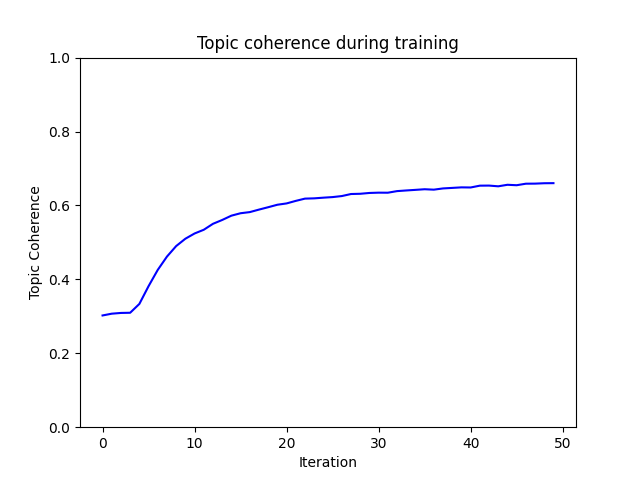
\includegraphics[width= \linewidth]{figures/pachinko_training.PNG}
	\caption{Topic coherence during training of the taxonomy-topic model.}
	\label{fig:pachinko_train}
\end{figure}

From sample documents written by the most similar author pair (Lars Termansen \& Mikkel Færgemann Viken), we find that both authors write a mix of regular news and sports articles.
Their high similarity could be due to the ratio between news and sports news for both authors being similar, and possibly also because of the types of news they write about.
Another interesting observation is that for the second most similar author pair (Morten Nis Klenø \& Anne Helene Thomsen) the difference in the number of articles written is significant.
Here Morten Nis Klenø has written just 17 articles while Anne Helene Thomsen has written 606 articles.
This suggests that some part of why these authors' similarity is high, simply depends on the types of news the authors have written, no matter the amount.

It is also worth noting that while authors that write scientific papers usually write in just a few subject areas, the scientific area they work in, this is not necessarily the case for news article authors.
In our dataset, this can be seen in the fact that the authors have written for 7.86 categories on average, with 7 categories as the median.
This can make it more difficult for the author-topic model to find patterns in what the authors write about, especially since each category can cover multiple topics.

A random selection of authors from the dataset and the top words from their most probable topic can be seen in \autoref{tab:author_top_words}.
